\documentclass[11pt,a4paper]{report}
\usepackage[textwidth=37em,vmargin=30mm]{geometry}
\usepackage{calc,xunicode,amsmath,amssymb,paralist,enumitem,tabu,booktabs,datetime2,xeCJK,xeCJKfntef,listings}
\usepackage{tocloft,fancyhdr,tcolorbox,xcolor,graphicx,eso-pic,xltxtra,xelatexemoji}

\newcommand{\envyear}[0]{2024}
\newcommand{\envdatestr}[0]{2024-10-15}
\newcommand{\envfinaldir}[0]{webdb/2024/20241015/final}

\usepackage[hidelinks]{hyperref}
\hypersetup{
    colorlinks=false,
    pdfpagemode=FullScreen,
    pdftitle={Web Digest - \envdatestr}
}

\setlength{\cftbeforechapskip}{10pt}
\renewcommand{\cftchapfont}{\rmfamily\bfseries\large\raggedright}
\setlength{\cftbeforesecskip}{2pt}
\renewcommand{\cftsecfont}{\sffamily\small\raggedright}

\setdefaultleftmargin{2em}{2em}{1em}{1em}{1em}{1em}

\usepackage{xeCJK,xeCJKfntef}
\xeCJKsetup{PunctStyle=plain,RubberPunctSkip=false,CJKglue=\strut\hskip 0pt plus 0.1em minus 0.05em,CJKecglue=\strut\hskip 0.22em plus 0.2em}
\XeTeXlinebreaklocale "zh"
\XeTeXlinebreakskip = 0pt


\setmainfont{Brygada 1918}
\setromanfont{Brygada 1918}
\setsansfont{IBM Plex Sans}
\setmonofont{JetBrains Mono NL}
\setCJKmainfont{Noto Serif CJK SC}
\setCJKromanfont{Noto Serif CJK SC}
\setCJKsansfont{Noto Sans CJK SC}
\setCJKmonofont{Noto Sans CJK SC}

\setlength{\parindent}{0pt}
\setlength{\parskip}{8pt}
\linespread{1.15}

\lstset{
	basicstyle=\ttfamily\footnotesize,
	numbersep=5pt,
	backgroundcolor=\color{black!5},
	showspaces=false,
	showstringspaces=false,
	showtabs=false,
	tabsize=2,
	captionpos=b,
	breaklines=true,
	breakatwhitespace=true,
	breakautoindent=true,
	linewidth=\textwidth
}






\newcommand{\coverpic}[2]{
    % argv: itemurl, authorname
    Cover photo by #2~~(\href{#1}{#1})
}
\newcommand{\makeheader}[0]{
    \begin{titlepage}
        % \newgeometry{hmargin=15mm,tmargin=21mm,bmargin=12mm}
        \begin{center}
            
            \rmfamily\scshape
            \fontspec{BaskervilleF}
            \fontspec{Old Standard}
            \fontsize{59pt}{70pt}\selectfont
            WEB\hfill DIGEST
            
            \vfill
            % \vskip 30pt
            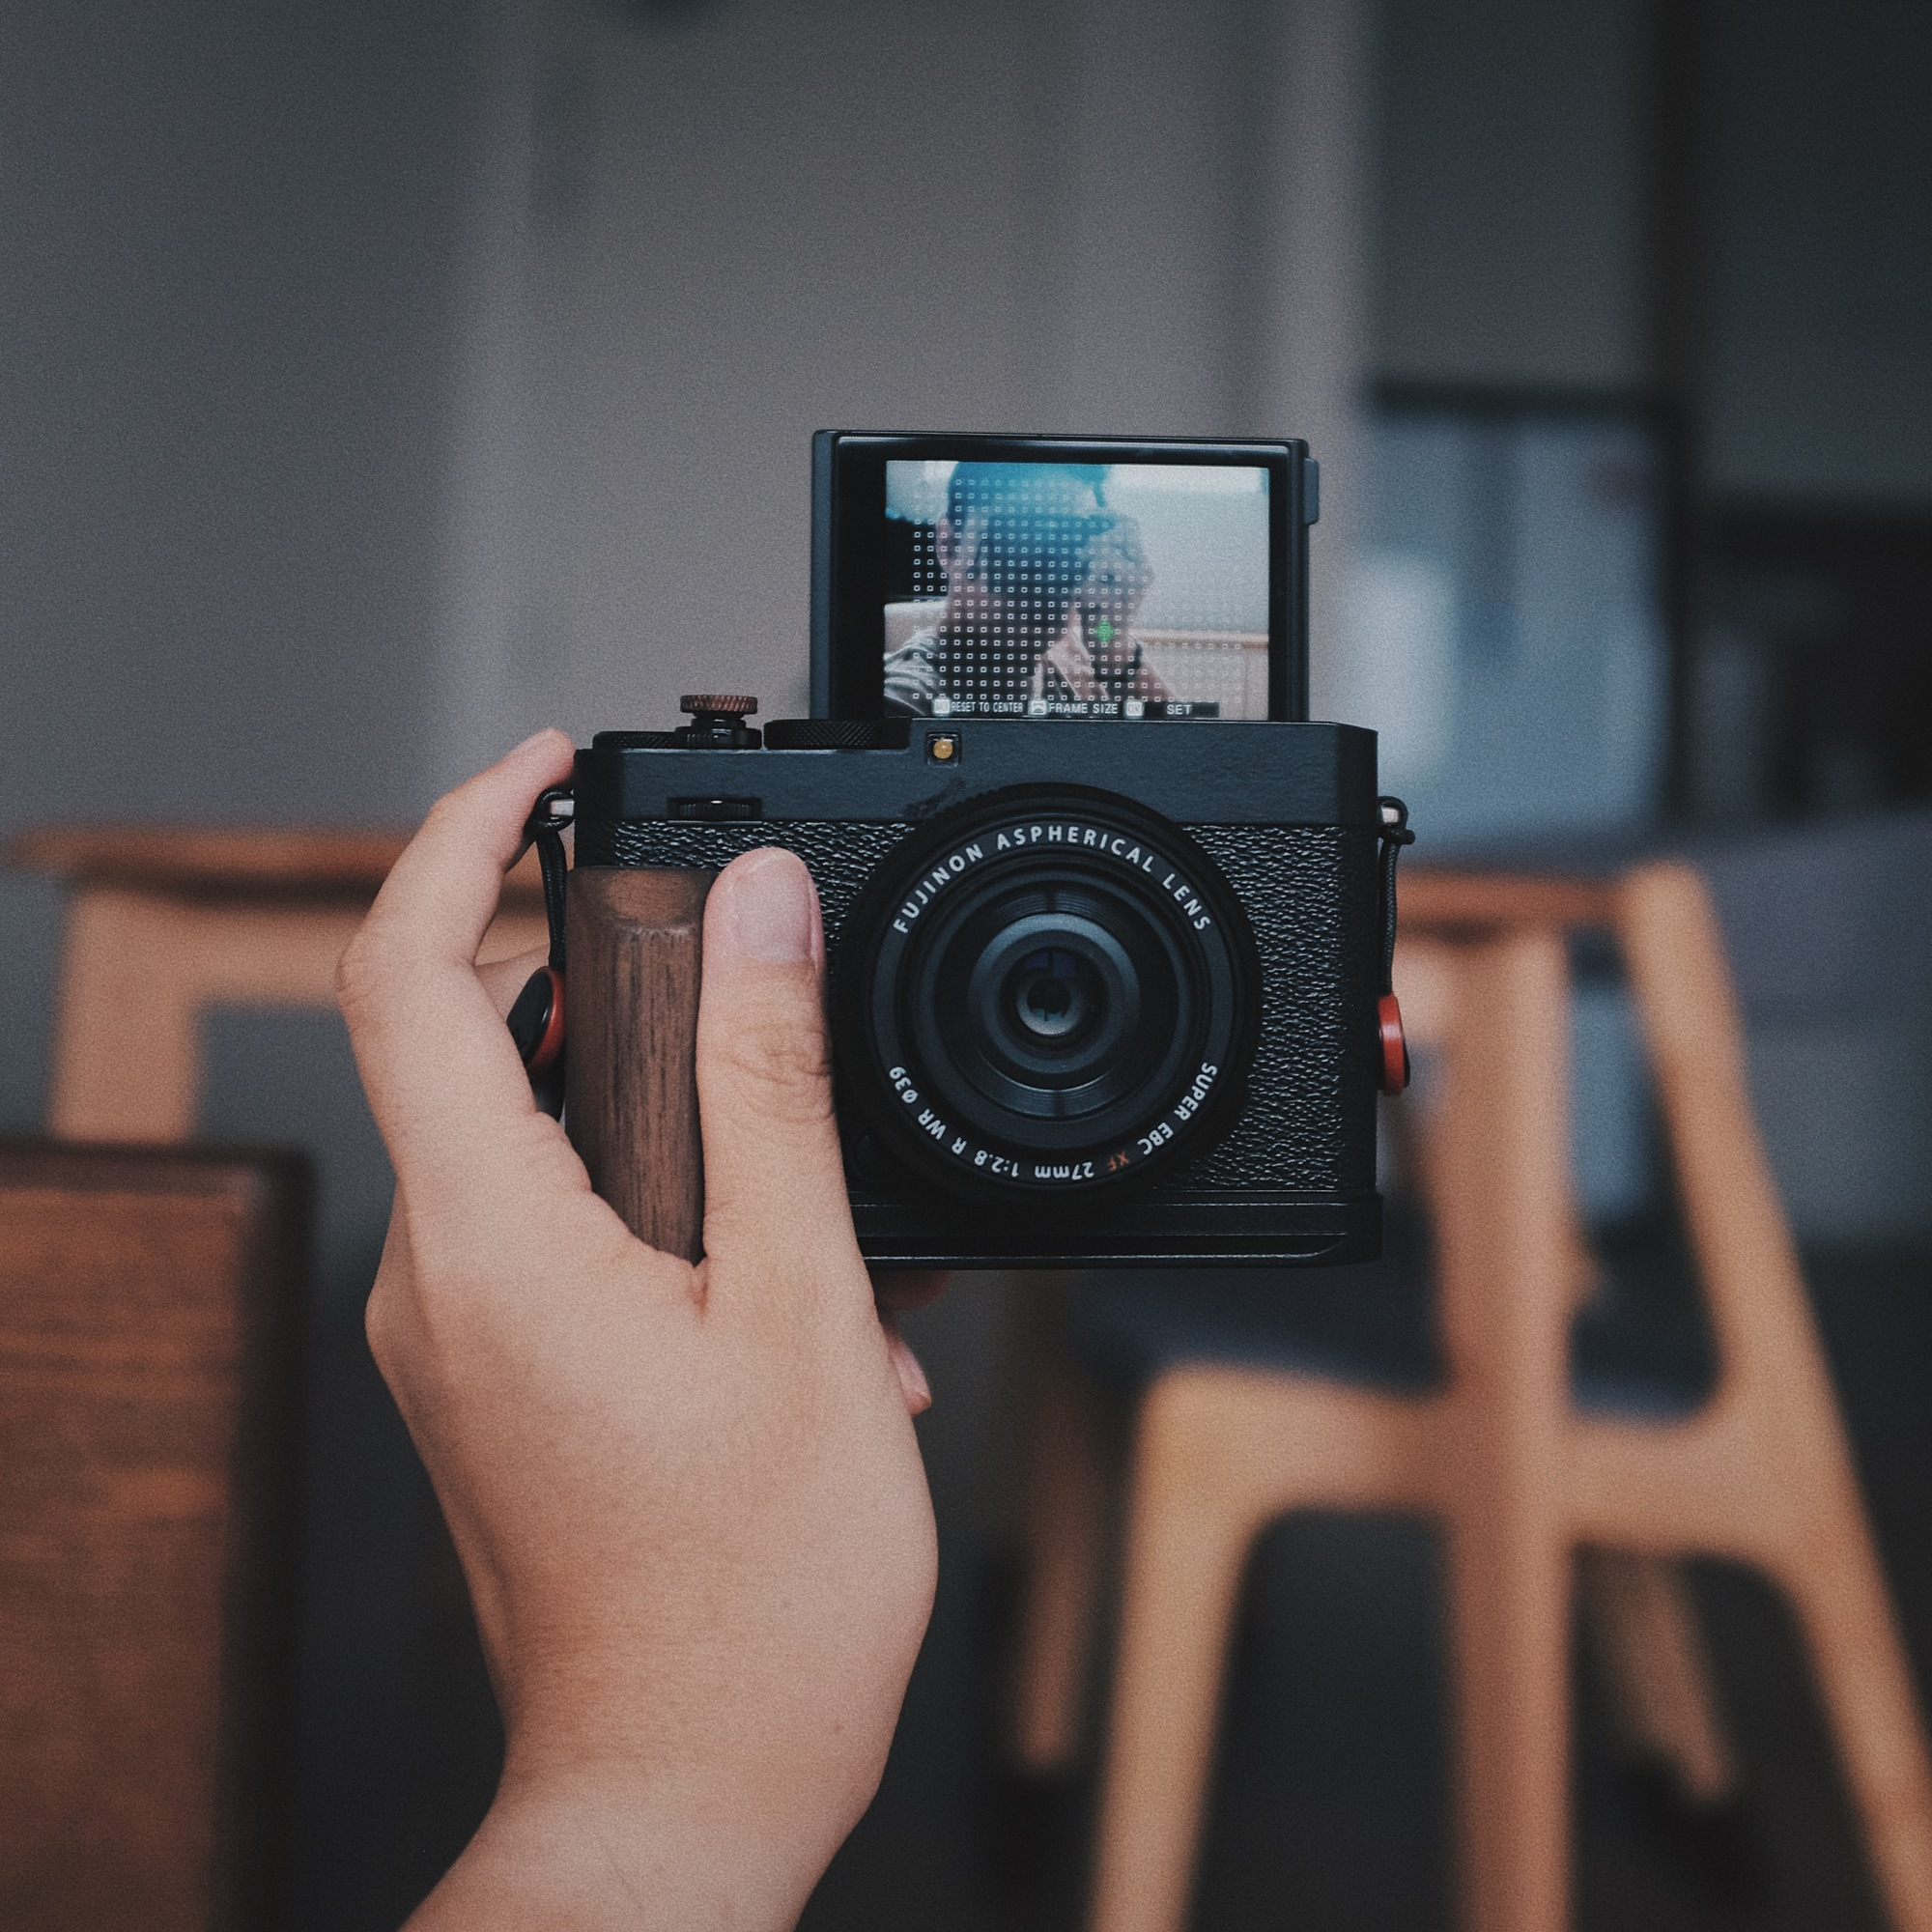
\includegraphics[width=\linewidth]{\envfinaldir/coverpic-prod.jpg}\par
            % \vskip 30pt
            \vfill

            \normalsize\rmfamily\scshape
            \copyright{} The Web Digest Project \hfill\large \envdatestr
        \end{center}
    \end{titlepage}
    % \restoregeometry
}
\newcommand{\simplehref}[1]{%
    \textcolor{blue!80!green}{\href{#1}{#1}}%
}
\renewcommand{\contentsname}{\center\Huge\sffamily\bfseries Contents\par\vskip 20pt}
\newcounter{ipartcounter}
\setcounter{ipartcounter}{0}
\newcommand{\ipart}[1]{
    % \vskip 20pt
    \clearpage
    \stepcounter{ipartcounter}
    \phantomsection
    \addcontentsline{toc}{chapter}{#1}
    % \begin{center}
    %     \Huge
    %     \sffamily\bfseries
    %     #1
    % \end{center}
    % \vskip 20pt plus 7pt
}
\newcounter{ichaptercounter}
\setcounter{ichaptercounter}{0}
\newcommand{\ichapter}[1]{
    % \vskip 20pt
    \clearpage
    \stepcounter{ichaptercounter}
    \phantomsection
    \addcontentsline{toc}{section}{\numberline{\arabic{ichaptercounter}}#1}
    \begin{center}
        \Huge
        \sffamily\bfseries
        #1
    \end{center}
    \vskip 20pt plus 7pt
}
\newcommand{\entrytitlefont}[1]{\subsection*{\raggedright\Large\sffamily\bfseries#1}}
\newcommand{\entryitemGeneric}[2]{
    % argv: title, url
    \parbox{\linewidth}{
        \entrytitlefont{#1}\par\vskip 5pt
        \footnotesize\ttfamily\mdseries
        \simplehref{#2}
    }\vskip 11pt plus 11pt minus 1pt
}
\newcommand{\entryitemGithub}[3]{
    % argv: title, url, desc
    \parbox{\linewidth}{
        \entrytitlefont{#1}\par\vskip 5pt
        \footnotesize\ttfamily\mdseries
        \simplehref{#2}\par\vskip 5pt
        \small\rmfamily\mdseries#3
    }\vskip 11pt plus 11pt minus 1pt
}
\newcommand{\entryitemAp}[3]{
    % argv: title, url, desc
    \parbox{\linewidth}{
        \entrytitlefont{#1}\par\vskip 5pt
        \footnotesize\ttfamily\mdseries
        \simplehref{#2}\par\vskip 5pt
        \small\rmfamily\mdseries#3
    }\vskip 11pt plus 11pt minus 1pt
}
\newcommand{\entryitemHackernews}[3]{
    % argv: title, hnurl, rawurl
    % \parbox{\linewidth}{
    %     \entrytitlefont{#1}\par\vskip 5pt
    %     \footnotesize\ttfamily\mdseries
    %     \simplehref{#3}\par
    %     \textcolor{black!50}{\href{#2}{#2}}
    % }\vskip 11pt plus 11pt minus 1pt
    \begin{minipage}{\linewidth}
            \entrytitlefont{#1}\par\vskip 5pt
            \footnotesize\ttfamily\mdseries
            \simplehref{#3}\par
            \textcolor{black!50}{\href{#2}{#2}}
    \end{minipage}\par\vskip 11pt plus 11pt minus 1pt
}







\begin{document}

\makeheader

\tableofcontents\clearpage




\ipart{Developers}
\ichapter{Hacker News}
\entryitemTwoLinks{Bike Manufacturers Are Making Bikes Less Repairable}{https://news.ycombinator.com/item?id=41840971}{https://www.ifixit.com/News/101675/bike-manufacturers-are-making-bikes-less-repairable}

\entryitemTwoLinks{How I Experience Web Today (2021)}{https://news.ycombinator.com/item?id=41840931}{https://how-i-experience-web-today.com}

\entryitemTwoLinks{Google Funding Construction of Seven U.S. Nuclear Reactors}{https://news.ycombinator.com/item?id=41840769}{https://www.wsj.com/business/energy-oil/google-nuclear-power-artificial-intelligence-87966624}

\entryitemTwoLinks{Commonly used arm positions can overestimate blood pressure readings: study}{https://news.ycombinator.com/item?id=41840023}{https://medicalxpress.com/news/2024-10-commonly-arm-positions-substantially-overestimate.html}

\entryitemTwoLinks{Response to DHH}{https://news.ycombinator.com/item?id=41839864}{https://ma.tt/2024/10/on-dhh/}

\entryitemTwoLinks{Show HN: Vortex – a high-performance columnar file format}{https://news.ycombinator.com/item?id=41839773}{https://github.com/spiraldb/vortex}

\entryitemTwoLinks{DeepSeek: Advancing theorem proving in LLMs through large-scale synthetic data}{https://news.ycombinator.com/item?id=41838589}{https://arxiv.org/abs/2405.14333}

\entryitemTwoLinks{NASA's Europa Clipper Launch}{https://news.ycombinator.com/item?id=41838420}{https://www.youtube.com/watch?v=lQToTWKwtuw}

\entryitemTwoLinks{Busy Status Bar}{https://news.ycombinator.com/item?id=41838337}{https://busy.bar/?hn}

\entryitemTwoLinks{Scientists successfully breed corals to improve their heat tolerance}{https://news.ycombinator.com/item?id=41837925}{https://phys.org/news/2024-10-scientists-successfully-corals-tolerance.html}

\entryitemTwoLinks{The Stallman Report}{https://news.ycombinator.com/item?id=41837782}{https://stallman-report.org/}

\entryitemTwoLinks{Show HN: X11 tool to share a screen area in any video meeting}{https://news.ycombinator.com/item?id=41837204}{https://github.com/splitbrain/clipscreen}

\entryitemTwoLinks{Upgrading Uber's MySQL Fleet}{https://news.ycombinator.com/item?id=41836748}{https://www.uber.com/en-JO/blog/upgrading-ubers-mysql-fleet/}

\entryitemTwoLinks{Blocking the "Sign in with Google" Prompt (2023)}{https://news.ycombinator.com/item?id=41835217}{https://superuser.com/questions/1773208/how-can-i-block-the-sign-in-with-google-prompt-on-websites}

\entryitemTwoLinks{Gosub – An open-source browser engine}{https://news.ycombinator.com/item?id=41835040}{https://github.com/gosub-io/gosub-engine}

\entryitemTwoLinks{Embedded Rust in Production?}{https://news.ycombinator.com/item?id=41834662}{https://blog.lohr.dev/embedded-rust}

\entryitemTwoLinks{Huly – Open-source project management platform}{https://news.ycombinator.com/item?id=41833902}{https://github.com/hcengineering/platform}

\entryitemTwoLinks{Why pay for a search engine}{https://news.ycombinator.com/item?id=41833833}{https://help.kagi.com/kagi/why-kagi/why-pay-for-search.html}

\entryitemTwoLinks{Rama on Clojure's terms, and the magic of continuation-passing style}{https://news.ycombinator.com/item?id=41833629}{https://blog.redplanetlabs.com/2024/10/10/rama-on-clojures-terms-and-the-magic-of-continuation-passing-style/}

\entryitemTwoLinks{Python client for the \$20 Colmi R02 smart ring}{https://news.ycombinator.com/item?id=41833200}{https://tahnok.github.io/colmi\_r02\_client/colmi\_r02\_client.html}\ichapter{Phoronix}
\entryitemGeneric{\hskip 0pt{}NVIDIA Is Helping To Improve Linux's Dynamic Display Mux Support For Laptops}{https://www.phoronix.com/news/NVIDIA-Dynamic-Display-Mux-2024}

\entryitemGeneric{\hskip 0pt{}AMD EPYC 9755 DDR5-4800 vs. DDR5-6000 Memory Performance}{https://www.phoronix.com/review/amd-epyc-9755-ddr5}

\entryitemGeneric{\hskip 0pt{}GCC 15 "Stage 1" Feature Development Ending Next Month}{https://www.phoronix.com/news/GCC-15-Stage-1-Ends-November}

\entryitemGeneric{\hskip 0pt{}CodeWeavers Working On Better Input Device Support For Proton Gaming}{https://www.phoronix.com/news/CodeWeavers-Better-Proton-Input}

\entryitemGeneric{\hskip 0pt{}Corsair Void Headset Driver Expected For Linux 6.13}{https://www.phoronix.com/news/Corsair-Void-Headset-Linux-6.13}

\entryitemGeneric{\hskip 0pt{}Inkscape 1.4 Brings Numerous Enhancements To This Vector Graphics Editor}{https://www.phoronix.com/news/Inkscape-1.4-Released}

\entryitemGeneric{\hskip 0pt{}Llamafile 0.8.14 Introduces New CLI Chatbot Interface}{https://www.phoronix.com/news/Llamafile-0.8.14}

\entryitemGeneric{\hskip 0pt{}Linux 6.12-rc3 Released With Some Late NTFS Driver Enhancements}{https://www.phoronix.com/news/Linux-6.12-rc3-Released}

\entryitemGeneric{\hskip 0pt{}Linux 6.13 To Drop Some Old \& No Longer Maintained Staging Drivers}{https://www.phoronix.com/news/Linux-6.13-Dropping-Old-Drivers}


\ipart{Developers~~~~(zh-Hans)}
\ichapter{Solidot}
\entryitemGeneric{\hskip 0pt{}NASA 发射欧罗巴快船探索木星卫星}{https://www.solidot.org/story?sid=79489}

\entryitemGeneric{\hskip 0pt{}Meta 研究员认为大模型比猫还蠢}{https://www.solidot.org/story?sid=79488}

\entryitemGeneric{\hskip 0pt{}大模型容易遭到越狱攻击}{https://www.solidot.org/story?sid=79487}

\entryitemGeneric{\hskip 0pt{}SpaceX 首次以抓取的方式回收 Starship 助推器}{https://www.solidot.org/story?sid=79486}

\entryitemGeneric{\hskip 0pt{}中国研究员称找到方法利用量子退火破解公钥加密}{https://www.solidot.org/story?sid=79485}

\entryitemGeneric{\hskip 0pt{}NASA 证实计划制定月球时间标准}{https://www.solidot.org/story?sid=79484}

\entryitemGeneric{\hskip 0pt{}周末锻炼与定期锻炼在降低疾病风险上的效果相同}{https://www.solidot.org/story?sid=79483}

\entryitemGeneric{\hskip 0pt{}保守派更可能反民主和支持独裁}{https://www.solidot.org/story?sid=79482}

\entryitemGeneric{\hskip 0pt{}日本卡西欧公司证实客户数据被盗}{https://www.solidot.org/story?sid=79481}

\entryitemGeneric{\hskip 0pt{}Imgur 不再将成人幽默归类为成人内容}{https://www.solidot.org/story?sid=79480}

\entryitemGeneric{\hskip 0pt{}AI PC 未提振 PC 需求}{https://www.solidot.org/story?sid=79479}

\entryitemGeneric{\hskip 0pt{}宝可梦游戏源代码泄露}{https://www.solidot.org/story?sid=79478}

\entryitemGeneric{\hskip 0pt{}Matt Mullenweg 接手了 WP Engine 的一个流行 WP 插件}{https://www.solidot.org/story?sid=79477}

\entryitemGeneric{\hskip 0pt{}志愿者想要保护维基百科免遭 AI 生成内容的入侵}{https://www.solidot.org/story?sid=79476}

\entryitemGeneric{\hskip 0pt{}上交所通过重启系统解决堵单问题}{https://www.solidot.org/story?sid=79475}

\entryitemGeneric{\hskip 0pt{}美国肥胖率开始下降}{https://www.solidot.org/story?sid=79474}

\entryitemGeneric{\hskip 0pt{}男子通过苹果 AI 的短信总结获悉分手的消息}{https://www.solidot.org/story?sid=79473}

\entryitemGeneric{\hskip 0pt{}苹果研究员发现大模型不能形式推理}{https://www.solidot.org/story?sid=79472}

\entryitemGeneric{\hskip 0pt{}Google 准备让用户在 Android 上运行 Linux 应用}{https://www.solidot.org/story?sid=79471}

\entryitemGeneric{\hskip 0pt{}广东教育厅短信平台被黑客入侵群发成人电影网站链接}{https://www.solidot.org/story?sid=79470}\ichapter{V2EX}
\entryitemGeneric{\hskip 0pt{}[macOS] 求移动硬盘数据恢复软件推荐}{https://www.v2ex.com/t/1080284}

\entryitemGeneric{\hskip 0pt{}[问与答] 长期闲置后,旧电脑/手机的正确密码会失效吗?}{https://www.v2ex.com/t/1080283}

\entryitemGeneric{\hskip 0pt{}[iPhone] 香港哪买日版 16 靠谱?}{https://www.v2ex.com/t/1080281}

\entryitemGeneric{\hskip 0pt{}[汽车] 大家有关注五菱最近要出的 K CAR 吗?}{https://www.v2ex.com/t/1080280}

\entryitemGeneric{\hskip 0pt{}[天黑以后] 20241014 午夜俱乐部}{https://www.v2ex.com/t/1080279}

\entryitemGeneric{\hskip 0pt{}[问与答] 淘宝直播触发 bug 变了鬼号还有得救吗}{https://www.v2ex.com/t/1080278}

\entryitemGeneric{\hskip 0pt{}[RSS] 做了一个关于资源分享的站点 follow 源,欢迎大家关注。}{https://www.v2ex.com/t/1080277}

\entryitemGeneric{\hskip 0pt{}[问与答] 必应搜索一直抽风,求解答🙏}{https://www.v2ex.com/t/1080276}

\entryitemGeneric{\hskip 0pt{}[摄影] 出一个京东新鲜的富士 X-T5 1650 套装}{https://www.v2ex.com/t/1080275}

\entryitemGeneric{\hskip 0pt{}[分享创造] 一个免费的工具集合 tooleasy.org}{https://www.v2ex.com/t/1080274}

\entryitemGeneric{\hskip 0pt{}[程序员] 单用户余额高并发支出收入有啥好方案?}{https://www.v2ex.com/t/1080273}

\entryitemGeneric{\hskip 0pt{}[问与答] pip 是怎么写的}{https://www.v2ex.com/t/1080272}

\entryitemGeneric{\hskip 0pt{}[求职] TypeScript 全栈开发求一份远程工作(全职或兼职,接单也可)}{https://www.v2ex.com/t/1080271}

\entryitemGeneric{\hskip 0pt{}[美酒与美食] 代糖与头痛}{https://www.v2ex.com/t/1080270}

\entryitemGeneric{\hskip 0pt{}[生活] 农村养老保险如何补缴}{https://www.v2ex.com/t/1080269}

\entryitemGeneric{\hskip 0pt{}[OpenWrt] 求助,网路旁路由问题}{https://www.v2ex.com/t/1080268}

\entryitemGeneric{\hskip 0pt{}[职场话题] 28 岁,金融外资的 BA 被 layoff 了,各位老哥们有啥过来人的智慧指点小弟一二}{https://www.v2ex.com/t/1080267}

\entryitemGeneric{\hskip 0pt{}[问与答] bat 脚本为什么总是打印出``系统找不到指定的驱动器。''?}{https://www.v2ex.com/t/1080266}

\entryitemGeneric{\hskip 0pt{}[Apple] 打算去香港入下个月新款 iPadmini7 和 macmini,是不是可以不丢盒子了?}{https://www.v2ex.com/t/1080265}

\entryitemGeneric{\hskip 0pt{}[计算机] 研一 求推荐笔记本 主要用来写深度学习代码}{https://www.v2ex.com/t/1080264}

\entryitemGeneric{\hskip 0pt{}[Apple] 这次是真羡慕安卓了,更好的性能更大的电池}{https://www.v2ex.com/t/1080262}

\entryitemGeneric{\hskip 0pt{}[SONY] 关于 sony 电视长期 cpu 高负载运行}{https://www.v2ex.com/t/1080259}

\entryitemGeneric{\hskip 0pt{}[Surge] Surge 托管配置问题请教}{https://www.v2ex.com/t/1080258}

\entryitemGeneric{\hskip 0pt{}[程序员] 求助,如何在反向代理的基础上实现 IP 轮换?}{https://www.v2ex.com/t/1080255}

\entryitemGeneric{\hskip 0pt{}[生活] 恰逢双 11+政府补贴+装修,想和大家交流下买家电的问题}{https://www.v2ex.com/t/1080254}

\entryitemGeneric{\hskip 0pt{}[iPhone] iPhone 钱包提示钱包中已有此卡}{https://www.v2ex.com/t/1080251}

\entryitemGeneric{\hskip 0pt{}[问与答] 在电脑屏幕上划线的工具叫什么,不截屏划}{https://www.v2ex.com/t/1080250}

\entryitemGeneric{\hskip 0pt{}[生活] 新买了辆车,又恰逢双十一,各位有没有什么车上的好东西分享推荐一下}{https://www.v2ex.com/t/1080248}

\entryitemGeneric{\hskip 0pt{}[酷工作] Data engineer and FSD 外企招聘 全英面试 base 广州}{https://www.v2ex.com/t/1080247}

\entryitemGeneric{\hskip 0pt{}[程序员] 聊一聊个人遇到职场上的问题,欢迎各位老哥来一起探讨}{https://www.v2ex.com/t/1080244}

\entryitemGeneric{\hskip 0pt{}[Kindle] Calibre 给 kindle 同步设置邮箱一直提示报错}{https://www.v2ex.com/t/1080243}

\entryitemGeneric{\hskip 0pt{}[Go 编程语言] 请教下有通信调度业务相关的 go 项目学习吗}{https://www.v2ex.com/t/1080242}

\entryitemGeneric{\hskip 0pt{}[问与答] 可以自己给显示器换屏吗?}{https://www.v2ex.com/t/1080241}

\entryitemGeneric{\hskip 0pt{}[macOS] 请教 MacOS 下 clashx 添加 vmess 单节点的方法}{https://www.v2ex.com/t/1080239}

\entryitemGeneric{\hskip 0pt{}[Java] Spring Aop 跨模块失效求助}{https://www.v2ex.com/t/1080238}

\entryitemGeneric{\hskip 0pt{}[Python] 其实我经常好奇一件事, 为什么 Python 得 dict 没有 set 方法, 有人知道什么历史原因吗}{https://www.v2ex.com/t/1080237}

\entryitemGeneric{\hskip 0pt{}[问与答] 杭州联通的宽带体验如何?}{https://www.v2ex.com/t/1080236}

\entryitemGeneric{\hskip 0pt{}[职场话题] 求助啊,不知道该准备什么内容}{https://www.v2ex.com/t/1080235}

\entryitemGeneric{\hskip 0pt{}[生活] 对未来和当下有些迷茫焦虑}{https://www.v2ex.com/t/1080234}

\entryitemGeneric{\hskip 0pt{}[酷工作] 纠结去哪个公司,希望有大佬帮忙指点一下}{https://www.v2ex.com/t/1080233}

\entryitemGeneric{\hskip 0pt{}[问与答] 安卓为啥禁止 app 联网,还是有流量统计呢}{https://www.v2ex.com/t/1080232}

\entryitemGeneric{\hskip 0pt{}[宽带症候群] 一个没有多余功能和不能改 SN LOID 的猫 账号密码正确但不能上网怎么办?}{https://www.v2ex.com/t/1080231}

\entryitemGeneric{\hskip 0pt{}[硬件] 双 11 攒机求指教}{https://www.v2ex.com/t/1080228}

\entryitemGeneric{\hskip 0pt{}[小米] 小米的冰箱可以买吗}{https://www.v2ex.com/t/1080227}

\entryitemGeneric{\hskip 0pt{}[问与答] 抉择 - 24 岁还是 30 岁}{https://www.v2ex.com/t/1080226}

\entryitemGeneric{\hskip 0pt{}[问与答] 你们是怎么分配使用公司电脑和自己电脑的}{https://www.v2ex.com/t/1080225}

\entryitemGeneric{\hskip 0pt{}[问与答] ios 设备实现群控必须要越狱吗}{https://www.v2ex.com/t/1080223}

\entryitemGeneric{\hskip 0pt{}[游戏] 双十一想换个 CPU 和主板,有推荐的吗}{https://www.v2ex.com/t/1080222}

\entryitemGeneric{\hskip 0pt{}[Apple] Mac 下 G502hero 的回报率问题}{https://www.v2ex.com/t/1080221}

\entryitemGeneric{\hskip 0pt{}[职场话题] H3C 防火墙目前最推荐的高可用方案是什么?}{https://www.v2ex.com/t/1080220}


\ipart{Generic News}
\ichapter{AP News}
\entryitemWithDescription{\hskip 0pt{}This camp provides a safe space for kids to learn and play after Hurricane Helene}{https://apnews.com/article/0125276a937ee77499c81afe9def39cd}{}\ichapter{Reuters}
\entryitemWithDescription{\hskip 0pt{}UK calls for restraint after China's military drills around Taiwan}{https://www.reuters.com/world/uk-calls-restraint-after-chinas-military-drills-around-taiwan-2024-10-14/}{Britain said on Monday it was concerned by China\textquotesingle s military exercises around Taiwan and said they increased tensions and risked "dangerous escalation" in the Taiwan...}

\entryitemWithDescription{\hskip 0pt{}EU ministers agree on COP29 negotiating position - official}{https://www.reuters.com/world/europe/eu-ministers-agree-cop29-negotiating-position-official-2024-10-14/}{EU environment ministers agreed on the bloc\textquotesingle s negotiating position ahead of the COP 29 United Nations climate summit in Azerbaijan next month, a council statement...}

\entryitemWithDescription{\hskip 0pt{}At least 12 killed, 33 injured in bus accident in Egypt, health ministry says}{https://www.reuters.com/world/africa/least-12-killed-33-injured-bus-accident-egypt-health-ministry-says-2024-10-14/}{At least 12 people were killed and 33 injured in Egypt on Monday after a bus overturned on a highway connecting Cairo to the Red Sea coast, the Egyptian health ministry...}

\entryitemWithDescription{\hskip 0pt{}Venezuela recognizes fiery ritual honoring goddess as cultural heritage}{https://www.reuters.com/world/americas/venezuela-recognizes-fiery-ritual-honoring-goddess-cultural-heritage-2024-10-14/}{Hundreds of bare-chested men circle flames on a dark night to the beat of drums in central Venezuela\textquotesingle s mountains. They dash across the blaze with bare feet over hot...}

\entryitemWithDescription{\hskip 0pt{}Canadian government says it has expelled six Indian diplomats and consular officials}{https://www.reuters.com/world/americas/canadian-government-says-it-has-expelled-six-indian-diplomats-consular-officials-2024-10-14/}{Canada has expelled six Indian diplomats and consular officials in relation to a targeted campaign against Canadian citizens by agents linked to the government of India, its foreign ministry said in a statement on...}

\entryitemWithDescription{\hskip 0pt{}Pentagon slams 'destabilizing' Chinese war games around Taiwan}{https://www.reuters.com/world/asia-pacific/pentagon-slams-destabilizing-chinese-war-games-around-taiwan-2024-10-14/}{The Pentagon on Monday strongly criticized Chinese military war games around Taiwan, calling them...}

\entryitemWithDescription{\hskip 0pt{}France calls for immediate release of French researcher jailed in Russia}{https://www.reuters.com/world/europe/france-calls-immediate-release-french-researcher-jailed-russia-2024-10-14/}{France called on Monday for the immediate release of French researcher Laurent Vinatier after he was found guilty by a Moscow court of breaking Russia\textquotesingle s "foreign agent" laws and sentenced to three years in...}

\entryitemWithDescription{\hskip 0pt{}China urges caution in Israel-Iran tensions, calls for ceasefire}{https://www.reuters.com/world/middle-east/china-urges-caution-israel-iran-tensions-calls-ceasefire-2024-10-14/}{Chinese Foreign Minister Wang Yi called on all parties involved in tensions between Israel and Iran on Monday to exercise caution and avoid escalating the...}

\entryitemWithDescription{\hskip 0pt{}Zelenskiy says he was briefed on N.Korean 'involvement' in Ukraine war}{https://www.reuters.com/world/europe/zelenskiy-says-he-was-briefed-nkorean-involvement-ukraine-war-2024-10-14/}{Ukrainian President Volodymyr Zelenskiy said on Monday he had been briefed about North Korea\textquotesingle s involvement in the war in his country and Russia\textquotesingle s plans for this autumn and...}

\entryitemWithDescription{\hskip 0pt{}World Health Organization receives \$1 billion in pledges for next budget}{https://www.reuters.com/business/healthcare-pharmaceuticals/world-health-organization-receives-1-billion-pledges-next-budget-2024-10-14/}{The World Health Organization said it received pledges worth \$700 million for its 2025-2028 budget at a event in Berlin on Monday, in addition to \$300 million already pledged by the European and African...}

\entryitemWithDescription{\hskip 0pt{}Mothers seek justice for minors detained in Venezuelan election aftermath}{https://www.reuters.com/world/americas/mothers-seek-justice-minors-detained-venezuelan-election-aftermath-2024-10-14/}{It was curiosity that drew 15-year-old Aliangel Jose Rodriguez to one of the protests that erupted following Venezuela\textquotesingle s contested presidential election in late July, his mother...}

\entryitemWithDescription{\hskip 0pt{}NASA launches spacecraft to gauge if Jupiter's moon Europa can host life}{https://www.reuters.com/science/nasa-launches-spacecraft-gauge-if-jupiters-moon-europa-can-host-life-2024-10-14/}{NASA launched a spacecraft from Florida on Monday on a mission to examine whether Jupiter\textquotesingle s moon Europa has conditions suitable to support life, with a focus on the large subsurface ocean believed to be lurking beneath its...}

\entryitemWithDescription{\hskip 0pt{}Ex-Stasi officer sentenced to 10 years in jail over 1974 Berlin Wall killing}{https://www.reuters.com/world/europe/ex-stasi-officer-sentenced-10-years-jail-over-1974-berlin-wall-killing-2024-10-14/}{A former officer for Communist East Germany\textquotesingle s Stasi secret police was sentenced to 10 years in prison on Monday for the fatal shooting of a Polish firefighter at a border crossing between East and West Berlin 50 years...}\ichapter{联合早报}
\entryitemWithDescription{沈泽玮:台湾冲突阻遏法案只叫不咬?}{https://www.zaobao.com/news/china/story20240918-4758889}{美国众议院9月9日开启了长达一星期的``中国周'',共通过25项主要涉华法案。(法新社) 美国众议院在当地时间9月9日开启了长达一星期的``中国周'',在美国总统和国会选举举行之前,密集表决数十项与中国有关的法案,共通过25项主要涉华法案……}

\entryitemWithDescription{欧盟电动车关税投票倒计时 中国在分歧中寻支持}{https://www.zaobao.com/news/china/story20240917-4758953}{欧盟27个成员国将于9月25日就是否继续对进口自中国的电动汽车额外征税进行最后表决。图为上海港等待装运出口的电动汽车。(彭博社) 欧盟对中国电动汽车加征关税的投票进入倒计时,正在欧洲访问的中国商务部部长王文涛与欧盟多国政府高层就此进行协商,试图在立场分歧的成员国中争取到更多支持。 受访学者研判,欧盟对中国电动汽车加征关税不可避免,但具体的加税方式和幅度仍有一定弹性,这是王文涛此行与各国谈判的重点……}

\entryitemWithDescription{港府今年将举办逾400项国庆活动}{https://www.zaobao.com/news/china/story20240917-4759341}{再过十多天就是中国国庆75周年,香港天星小轮展示``国庆75周年''\,``三天免费搭小轮''等标语迎国庆。(中新社) 再过十多天就是中国国庆75周年,香港特区政府今年将举办逾400项庆祝活动,希望通过一连串活动庆祝国庆,并且弘扬爱国主义教育及刺激消费。 港府星期二(9月17日)召开记者会,介绍各项庆祝国庆活动和特别优惠,涉及出行及吃喝玩乐等领域……}

\entryitemWithDescription{美空军部长:中国大陆军演精密化 为入侵封锁台湾做准备}{https://www.zaobao.com/news/china/story20240917-4759407}{美国空军部长肯德尔星期一(9月16日)在空军暨太空军协会的一场大会上致辞,提到中国对印太地区日益增长的威胁。(取自美国国防部网站) (华盛顿综合讯)美国空军部长肯德尔指,中国大陆军演的规模越来越大,也更加精密化,这是在专门为入侵、封锁台湾做准备。他也称,中国对印太地区的威胁现在已存在……}

\entryitemWithDescription{批准潜在对台备件军售案后 美派巡逻机过航台海}{https://www.zaobao.com/news/china/story20240917-4758770}{台军士兵8月26日在屏东县枋山训练场进行实弹演习时,从M1167 TOW运载车上发射一枚美制TOW-2A线导反坦克导弹。(路透社) (华盛顿/台北/北京综合讯)在批准潜在对台备件军售案之后,美国派遣反潜巡逻机过航台湾海峡,中国人民解放军东部战区则组织战机跟监美机,并誓言``坚决捍卫国家主权''……}

\entryitemWithDescription{李家超:若香港驻美经贸办被关 受害的是美企}{https://www.zaobao.com/news/china/story20240917-4758797}{香港特首李家超星期一(9月17日)警告,如果美国通过法案,导致香港驻美经贸办关闭,受害的是美国企业。图为李家超9月11日在``一带一路''高峰论坛上致辞。(彭博社) (香港综合讯)香港特首李家超警告,如果美国通过法案,导致香港驻美经贸办关闭,受害的是美国企业。 美国众议院上周通过《香港经济贸易办事处认证法案》,如果参议院也表决通过并交由总统签署成法,香港三个驻美国的经贸办可能将被强制关闭……}

\entryitemWithDescription{美国指中国航空工业集团员工企图实施黑客攻击}{https://www.zaobao.com/news/china/story20240917-4757988}{(华盛顿综合讯)中国航空航天巨头中国航空工业集团一名员工被指试图对美国宇航局、美国军方和其他目标展开黑客攻击。 据彭博社报道,美国检察官布坎南星期一(9月16日)在起诉书中,指控中国航空工业集团39岁的工程师吴宋(音译,Song Wu)企图从美国宇航局、空军、陆军和海军,以及联邦航空管理局取得电脑软件和源代码……}

\entryitemWithDescription{【东谈西论】恒大账务造假 普华永道是共犯还是被拖累?}{https://www.zaobao.com/news/china/story20240917-4756452}{因涉及恒大地产审计项目的违法行为,普华永道中国9月13日被中国财政部和证监会处以4.41亿人民币罚款并被令停业六个月, 广州分所被撤销……}

\entryitemWithDescription{戴庆成:香港输入人才计划大检阅}{https://www.zaobao.com/news/china/story20240917-4744978}{香港于2022年底推出高端人才通行证计划。(法新社) 2019年香港反修例风波过后,数以十万计港人移居海外,令香港出现人才荒。港府为了解决这个问题,在过去几年积极引入``新血'',当中以高才通计划最受瞩目,社会上也不时热议其成效。 高才通全称为高端人才通行证计划,于2022年底推出,申请人年收入须达到250万港元(约42万新元)以上,或本科毕业于全球百强大学并满足一定工作年限等……}

\entryitemWithDescription{中美希望稳定双边关系 中小国家可​​​搭建桥梁}{https://www.zaobao.com/news/china/story20240917-4745091}{中美元首去年11月在旧金山会晤后,双方都希望稳定两国关系,我国巡回大使陈庆珠认为,如果中美两国都认为走向战争不符合它们的利益,那么中小国家就可以做点什么,为双方搭建桥梁。 陈庆珠星期一(9月16日)在李光耀公共政策学院的一场研讨会上说,中国与西方的关系面对诸多困难,有中国智库表示,希望新加坡能协助在中美之间建立更多对话,``因为新加坡受美国信任,也在中国有渠道''……}

\entryitemWithDescription{陈庆珠:世界经历了三次``中国冲击'' 中美的主导力之争将继续}{https://www.zaobao.com/news/china/story20240917-4744996}{李光耀公共政策学院``思想之节庆''的一场研讨会,讨论``历史终结时的中国冲击''。左起是我国巡回大使陈庆珠、通商中国主席李奕贤、李光耀公共政策学院国际关系助理教授何莉菁、李光耀公共政策学院院长柯成兴……}

\entryitemWithDescription{上海遭遇75年来最强台风 扰乱民众中秋假期出行}{https://www.zaobao.com/news/china/story20240916-4745224}{台风贝碧嘉星期一(9月16日)登陆上海,维护人员星期一下午在衡山路上处理倒伏的树木。 (新华社) 台风造成上海上万株数目倒伏或折断。图为一棵倒下的大树砸坏一旁的建筑。(法新社) 台风贝碧嘉登陆上海后,黄浦江苏州河口潮位上涨,乌云密布。(中新社) 中国上海市星期一(9月16日)遭遇75年来最强台风``贝碧嘉''登陆,也是上海有记录以来首次有强台风侵袭……}

\entryitemWithDescription{陆男频长驱偷渡台湾在测试边防实力?}{https://www.zaobao.com/news/china/story20240916-4745161}{中国大陆一名王姓男子在中秋节前夕,乘橡皮艇从浙江宁波抵达台湾新北市林口,主动打电话投案,海巡署人员前去接他上岸。(自由時報) 中国大陆一名王姓男子划橡皮艇于上星期六清晨偷渡到台湾,隔天被新北市地方法院裁定羁押禁见。这是6月以来第二起大陆人士偷渡至台湾,此间专家质疑是否为海防破口,并怀疑对岸是否在测试台湾的边防实力……}

\entryitemWithDescription{中美时隔八月举行国防部工作会晤}{https://www.zaobao.com/news/china/story20240916-4745025}{(北京/华盛顿综合讯)中美双方上周末举行国防部工作会晤;美国官员称,美国积极进行美中两军外交活动,不代表美国对有关中国议题的处理方式发生任何改变。 据中国国防部星期天(15日)晚上通报,北京香山论坛结束后,第18次中美国防部工作会晤上星期六至星期天(9月14日至15日)在北京举行……}

\entryitemWithDescription{中国高校今年拟增足球运动本科专业}{https://www.zaobao.com/news/china/story20240916-4744925}{(北京综合讯)为了培养足球专业人才,中国大专学府今年度拟新增足球运动本科专业,以具体落实中国足球改革。 综合人民网和《南方都市报》报道,中国教育部上星期五(9月13日)发布《2024年度普通高等学校本科专业申报材料公示》。根据公示统计,今年度拟新增专业535个,涉及353所高校,其中39所高校新增足球运动专业……}

\entryitemWithDescription{香港23条首案 港男因穿``光时''上衣被定罪}{https://www.zaobao.com/news/china/story20240916-4743439}{(香港综合讯)香港一名无业男子,今年6月因穿印有2019年反修例抗争口号的上衣而被捕。他星期一承认违反煽动意图罪,成为在《维护国家安全条例》(即《香港基本法》第23条)下被定罪的第一人。 综合港媒《星岛日报》和路透社报道,27岁无业男子诸启邦今年6月12日在石门港铁站附近,未能出示身份证供查阅被警方拘捕……}

\entryitemWithDescription{美国务院:中国释放被关押近20年美籍牧师}{https://www.zaobao.com/news/china/story20240916-4744614}{(华盛顿综合电)中国释放被关押近20年的美国籍牧师,显示北京在中美关系的关键时刻展现善意。 综合彭博社、法新社和路透社报道,美国国务院发言人星期天(9月15日)说:``我们欢迎林大卫(音译,David Lin)从中华人民共和国的监狱获释。他已回返美国,这是他近20年来首次与家人见面。'' 林大卫的女儿艾丽斯告诉美国政治新闻网Politico,她的父亲将抵达得克萨斯州的圣安东尼奥……}

\entryitemWithDescription{中国驻泰使馆:近期并未向湄公河下游泄洪}{https://www.zaobao.com/news/china/story20240916-4743917}{(北京讯)泰国西北部的湄公河因洪水泛滥而决堤,中国否认这是中方泄洪所致,并称近来已持续减少云南景洪水电站的出库流量,以助下游地区抗洪。 中国驻泰国大使馆星期日(9月15日)深夜在官方微信公众号发文说,当天又有媒体报道称中国正在向湄公河泄洪,经向中国主管部门核实,使馆再次澄清,为帮助下游地区应对洪灾,中方近来持续稳定和减少景洪水电站出库流量,不可能对下游地区抗洪救灾形成压力……}

\entryitemWithDescription{加入美国储存可靠度评估计划 台湾军方编列预算采购三类型导弹}{https://www.zaobao.com/news/china/story20240916-4743826}{(台北讯)据台媒报道,台湾军方持续向美国采购可简易操作的导弹,预计在2024年、2031年以前获得400枚``标枪''反装甲导弹、2485枚``刺针''人携式防空导弹……}

\entryitemWithDescription{韩咏红:中美分头追逐全球南方}{https://www.zaobao.com/news/china/story20240916-4730719}{9月5日,中国外长王毅(中)同中非合作论坛非方现任共同主席国塞内加尔外长法勒(左)、下任共同主席国刚果外长加科索(右),在北京共同会见中外记者并答问。(路透社) 进入气候宜人的9月,中国接连举行了两场受瞩目的国际会议,一是聚集非洲53国国家元首与政要的中非合作论坛,接着是周末刚闭幕的北京香山论坛。 两场活动的参与者不同,规模也有很大差距……}

\entryitemWithDescription{菲律宾船只撤离中菲争议海域后 将再派船接替}{https://www.zaobao.com/news/china/story20240915-4730494}{这张在9月15日拍摄,并由菲律宾海岸警卫队提供的照片显示,菲律宾海岸警卫队船马格巴努亚号抵达了菲国巴拉望岛的一个港口。菲律宾早前以发现填海活动为由,今年4月派出马格巴努亚号前往萨比纳礁。(法新社/菲律宾海岸警卫队) 菲律宾国家海事委员会星期天(9月15日)发声明称,该国海岸警卫队一艘巡逻舰已离开萨比纳礁争议海域……}

\entryitemWithDescription{台风贝碧嘉直击中国华东 多趟本地与沪杭间航班取消}{https://www.zaobao.com/news/china/story20240915-4730611}{9月15日在上海外滩滨江步道上,一名外籍游客的雨伞被大风吹起。台风贝碧嘉的中心当天下午5时位于上海市东偏南方大约435公里的东海海面上,中心附近最大风力有13级。(中新社) (上海/新加坡综合讯)台风贝碧嘉预计将为中国华东沿海地区带来狂风暴雨,多趟往返新加坡与上海和杭州的航班取消……}






\clearpage
\leavevmode\vfill
\footnotesize

Copyright \copyright{} 2023-2024 Neruthes and other contributors.

This document is published with CC BY-NC-ND 4.0 license.

The entries listed in this newsletter may be copyrighted by their respective creators.

This newsletter is generated by the Web Digest project.

The newsletters are also delivered via Telegram channel \CJKunderline{\href{https://t.me/webdigestchannel}{https://t.me/webdigestchannel}}.\\
RSS feed is available at \CJKunderline{\href{https://webdigest.pages.dev/rss.xml}{https://webdigest.pages.dev/rss.xml}}.

This newsletter is available in PDF at
\CJKunderline{\href{https://webdigest.pages.dev/}{https://webdigest.pages.dev/}}.

The source code being used to generate this newsletter is available at\\
\CJKunderline{\href{https://github.com/neruthes/webdigest}{https://github.com/neruthes/webdigest}}.

This newsletter is also available in
\CJKunderline{\href{http://webdigest.pages.dev/readhtml/\envyear/WebDigest-20241015.html}{HTML}} and
\CJKunderline{\href{https://github.com/neruthes/webdigest/blob/master/markdown/\envyear/WebDigest-20241015.md}{Markdown}}.


\coverpic{https://unsplash.com/photos/a-winding-road-in-the-middle-of-a-mountain-range-poyjT5Ap-oM}{Andrei R. Popescu}


\end{document}
